\documentclass[12pt]{extarticle}

\usepackage{tabularx}
\usepackage{amsmath}
\usepackage{extsizes}
\usepackage{graphicx}
\usepackage{amssymb}
\usepackage[english,russian]{babel}
\usepackage[utf8]{inputenc}
\usepackage[a4paper]{geometry}
\geometry{top=20mm,bottom=30mm,left=20mm,right=15mm}
\usepackage[T1,T2A]{fontenc}
\usepackage{setspace}
\usepackage{indentfirst}
\usepackage{caption}
\renewcommand{\baselinestretch}{1.5}
\usepackage{spverbatim}
\usepackage{listings}
\usepackage{xcolor}
\usepackage{tabularray}

\lstset{extendedchars=\true}
\definecolor{codebg}{gray}{0.96}
\definecolor{comment}{gray}{0.45}
\definecolor{keyword}{RGB}{0, 75, 150}
\definecolor{string}{RGB}{150, 80, 30}
\definecolor{number}{gray}{0.5}
\definecolor{identifier}{rgb}{0,0,0}

\lstdefinestyle{coolprint}{
  basicstyle   = \ttfamily\footnotesize,
  keywordstyle = \bfseries\color{keyword},
  commentstyle = \itshape\color{comment},
  stringstyle  = \color{string},
  identifierstyle = \color{identifier},
  backgroundcolor = \color{codebg},
  numbers      = left,
  numberstyle  = \footnotesize\color{number},
  numbersep    = 5pt,
  frame        = single,
  framerule    = 0.8pt,
  framesep     = 3pt,
  breaklines   = true,
  breakatwhitespace = true,
  tabsize      = 4,
  showspaces   = false,
  showstringspaces = false,
  showtabs     = false,
  xleftmargin  = 10pt,
  xrightmargin = 5pt,
  aboveskip    = \medskipamount,
  belowskip    = \medskipamount,
  captionpos   = b,
}
\lstset{style=coolprint}

\begin{document}

\begin{center}
  \textbf{МИНОБРНАУКИ РОССИИ} \\
  \textbf{Санкт-Петербургский государственный} \\
  \textbf{электротехнический университет} \\
  \textbf{«ЛЭТИ» им. В.И. Ульянова (Ленина)} \\
  \textbf{Кафедра ВТ} \\
\end{center}

\vspace{0.25\textheight}

\begin{center}
\textbf{ОТЧЕТ} \\
\textbf{по лабораторной работе №3} \\
\textbf{по дисциплине «ОргЭВМиС»} \\
\textbf{Тема: РАБОТА С ПЕРИФЕРИЙНЫМИ УСТРОЙСТВАМИ В RIPES} \\
\end{center}

\vspace*{\fill}

\begin{center}
\begin{tabularx}{\textwidth}{ l X r }
 Студенты гр. 5352 & \rule{8cm}{0.2mm} & Соболевский М.А. \\
 & \rule{8cm}{0.2mm} & Решетников С.А. \\
 Преподаватель & \rule{8cm}{0.2mm} & Кочетков А.В. \\
\end{tabularx}
\end{center}

\vspace{3em}

\begin{center}
Санкт-Петербург\\
\the\year
\end{center}

\thispagestyle{empty}

\pagebreak

\section{Задание на лабораторную работу}

Вариант №8.

\begin{enumerate}
    \item Изучить симуляцию светодиодной матрицы с использованием программы на ассемблере \texttt{leds\_new.s}. Для фрагмента кода (метка начала \texttt{nextRow}, метка завершения \texttt{nextPixel}) сформулировать результаты анализа в табличной форме (2 столбца: инструкция + назначение).
    \item Симуляция светодиодной матрицы с использованием программы на C \texttt{leds\_new.c}. Изменить код в соответствии с вариантом:
    \begin{itemize}
        \item размер матрицы: 7×5 ;
        \item отображаемая фигура: бирюзовая горизонтальная пунктирная линия;
        \item фон: отсутствие подсветки (чёрный).
    \end{itemize}
    \item Симуляция переключения светодиодов с использованием программы на C \texttt{switchesAndLeds.c}. Изменить код в соответствии с вариантом:
    \begin{itemize}
        \item размер матрицы: 8×3;
        \item число переключателей: 8;
        \item порядок подключения: \(0\to7, 1\to6, \ldots, 7\to0\);
        \item порядок цветов после включения всех светодиодов: b-r-g-b-r-g-b-r (синий, красный, зелёный, синий, красный, зелёный, синий, красный).
    \end{itemize}
\end{enumerate}

\section{Текст программы}

\subsection{Фрагмент программы \texttt{leds\_new.s} для анализа}
\renewcommand{\baselinestretch}{1}
\begin{lstlisting}[language={[x86masm]Assembler},caption={Фрагмент \texttt{nextRow}--\texttt{nextPixel} из \texttt{leds\_new.s}}]
nextRow:
    mv   a4, zero
    slli a3, t1, 8
    sub  a3, a3, t1
    divu a3, a3, a2
    slli a3, a3, 8
    and  t5, a3, a7
    mv   a5, t2
    mv   a3, a1
nextPixel:
    divu s0, a4, a1
    add  s1, t4, a4
    divu s1, s1, t3
    slli s0, s0, 16
    and  s0, s0, t0
    or   s0, t5, s0
    andi s1, s1, 255
    or   s0, s0, s1
    sw   s0, 0(a5)
    addi a3, a3, -1
    addi a5, a5, 4
    addi a4, a4, 255
    bnez a3, nextPixel
\end{lstlisting}
\renewcommand{\baselinestretch}{1.5}

\subsection{Изменённая программа \texttt{leds\_new.c}}
\renewcommand{\baselinestretch}{1}
\input{assets/leds_new}
\renewcommand{\baselinestretch}{1.5}

\subsection{Изменённая программа \texttt{switchesAndLeds.c}}
\renewcommand{\baselinestretch}{1}
\input{assets/switchesAndLeds}
\renewcommand{\baselinestretch}{1.5}

\section{Анализ фрагмента программы \texttt{leds\_new.s}}

\begin{longtblr}{colspec={|l|X|}, hlines, vlines}
\textbf{Инструкция} & \textbf{Назначение в контексте программы} \\
\texttt{mv a4, zero} & Обнуление счётчика пикселей в строке. \\
\texttt{slli a3, t1, 8} & \(a3 \leftarrow t1 \ll 8\) (умножение номера строки на 256). \\
\texttt{sub a3, a3, t1} & \(a3 \leftarrow a3 - t1 = t1 \cdot 255\). \\
\texttt{divu a3, a3, a2} & Деление на высоту матрицы (a2) для вычисления компоненты цвета. \\
\texttt{slli a3, a3, 8} & Сдвиг на 8 бит для размещения компоненты в нужной позиции. \\
\texttt{and t5, a3, a7} & Маскирование для выделения нужных битов цвета. \\
\texttt{mv a5, t2} & Загрузка текущего адреса LED-матрицы в a5. \\
\texttt{mv a3, a1} & Инициализация счётчика пикселей в строке (a1 — ширина). \\
\texttt{divu s0, a4, a1} & Вычисление номера строки для текущего пикселя (a4/a1). \\
\texttt{add s1, t4, a4} & Сложение для формирования байта цвета. \\
\texttt{divu s1, s1, t3} & Деление для получения компоненты синего цвета. \\
\texttt{slli s0, s0, 16} & Сдвиг красной компоненты в старшие 8 бит. \\
\texttt{and s0, s0, t0} & Маскирование красной компоненты. \\
\texttt{or s0, t5, s0} & Объединение с зелёной компонентой. \\
\texttt{andi s1, s1, 255} & Выделение младших 8 бит синей компоненты. \\
\texttt{or s0, s0, s1} & Формирование итогового 24-битного цвета. \\
\texttt{sw s0, 0(a5)} & Запись цвета в текущий пиксель LED-матрицы. \\
\texttt{addi a3, a3, -1} & Уменьшение счётчика пикселей. \\
\texttt{addi a5, a5, 4} & Переход к следующему пикселю (адрес + 4). \\
\texttt{addi a4, a4, 255} & Увеличение смещения для вычисления цвета. \\
\texttt{bnez a3, nextPixel} & Повтор цикла, пока не обработаны все пиксели строки. \\
\end{longtblr}

\section{Примеры запуска программ и снимки экрана}

\subsection{Настройка периферии и запуск}

Для выполнения работы в Ripes были созданы необходимые периферийные устройства:
\begin{itemize}
    \item для программы \texttt{leds\_new.s} — LED Matrix с параметрами Height=5, Width=7, увеличенный LED Size;
    \item для программы \texttt{leds\_new.c} — LED Matrix с параметрами Height=3, Width=8;
    \item для программы \texttt{switchesAndLeds.c} — LED Matrix (Height=3, Width=8) и Switches (8 переключателей).
\end{itemize}

Компиляция C-программ выполнялась с использованием настроенного кросс-компилятора RISC-V. Запуск производился в режиме Autoclock (F6) и пошагово (Clock, F5).

\subsection{Скриншоты}

\begin{center}
    \textbf{Работа программы \texttt{leds\_new.s} (матрица 5×7):}

    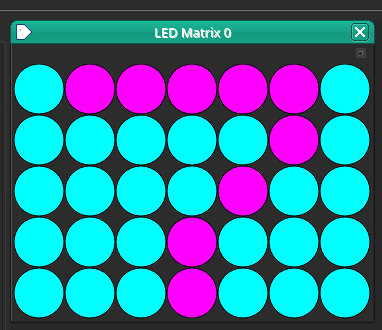
\includegraphics[width=0.4\textwidth]{assets/Pasted image.png}
\end{center}

\begin{center}
    \textbf{Работа изменённой программы \texttt{switchesAndLeds.c} (матрица 8×3, переключатели выключены):}

    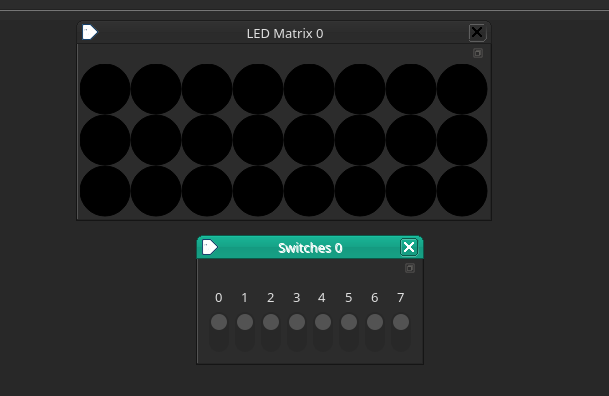
\includegraphics[width=0.4\textwidth]{assets/Pasted image (3).png}
\end{center}

\begin{center}
    \textbf{Работа изменённой программы \texttt{switchesAndLeds.c} (все переключатели включены):}

    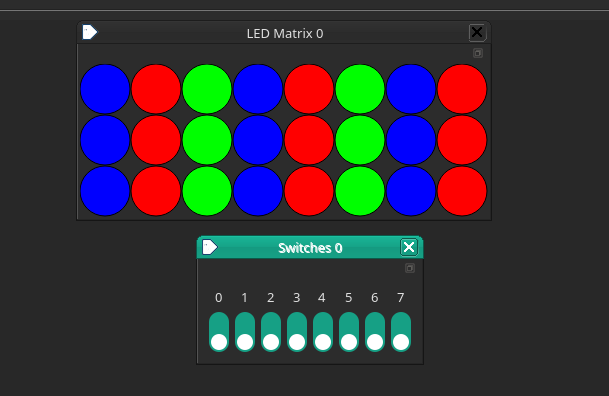
\includegraphics[width=0.4\textwidth]{assets/Pasted image (2).png}
\end{center}

\begin{center}
    \textbf{Работа изменённой программы \texttt{switchesAndLeds.c} (часть переключателей включена включены):}

    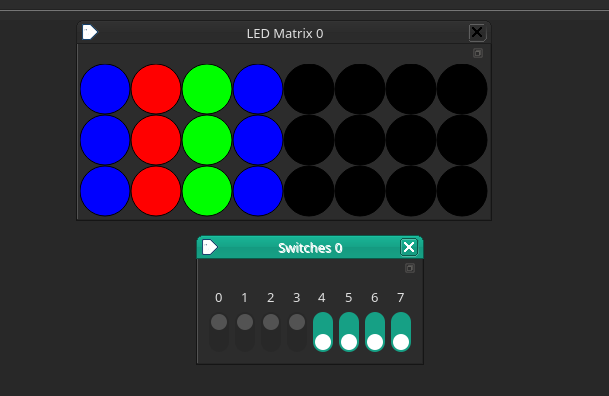
\includegraphics[width=0.4\textwidth]{assets/Pasted image (4).png}
\end{center}

\section{Выводы}

В ходе лабораторной работы были изучены методы работы с периферийными устройствами в симуляторе Ripes: светодиодной матрицей и переключателями. 

Была проанализирована программа на ассемблере \texttt{leds\_new.s}. Для фрагмента \texttt{nextRow}--\texttt{nextPixel} составлена таблица, поясняющая назначение каждой инструкции. Анализ показал, что данный фрагмент реализует вычисление цвета пикселя на основе его координат и запись значения в память LED-матрицы.

Программа \texttt{leds\_new.c} была изменена в соответствии с вариантом задания: матрица 8×3, отображается бирюзовая горизонтальная пунктирная линия на чёрном фоне. Программа успешно скомпилирована и запущена, результат наблюдается на LED-матрице.

Программа \texttt{switchesAndLeds.c} также была доработана под вариант: матрица 8×3, 8 переключателей, обратный порядок подключения (\(0\to7, 1\to6, \ldots, 7\to0\)) и заданная последовательность цветов b-r-g-b-r-g-b-r. При включении переключателей соответствующие столбцы матрицы загораются нужными цветами.

Все поставленные задачи выполнены, получены навыки настройки периферии, компиляции и отладки программ в Ripes.

\end{document}
